% answers.tex —— 1977 年·江苏苏州市初试卷 · 参考答案与详细解析片段
% 由 tools/generate_projects.py 依来源总账自 1977/1977_数学真题_江苏苏州市初试_试题.md + 1977/1977_数学真题_江苏苏州市初试_解析正文.md + 1977/1977_数学真题_江苏苏州市初试_答案要点.md 生成，勿手改（改源 MD 后重跑）


\begin{gktip}
固定源为三页纯题面扫描（原书页码 236 起），未附解答。下文各题由编者独立推导。原卷大题号「一、……六、」已转写为阿拉伯数字；大题一内 12 个小题原用阿拉伯数字「1．2．…12．」编号，统一转写为「（N）」。附加题按源卷自身编号（1、2）接排在第 6 题解析之后。
\end{gktip}

\begin{answer}
\gksolhead{1}{}

\textbf{题目}（每小题 5 分）：

\Needspace{5\baselineskip}
（1） 计算：

\nopagebreak[4]
\[
1\div\left(-\frac18\right)^2\times\left(-\frac14\right)^3+\left(-1\frac13\right)^2\div\left(\frac23\right)^2.
\]

（2） 已知：$3:x=6:y$，求 $\dfrac{x}{y}=?$

（3） 若 $\sqrt{(3-x)^2}=x-3$ 成立，求 $x$ 的取值范围。

（4） 求函数 $y=\dfrac{1}{2x^2-5x-3}$ 的自变量 $x$ 的取值范围。

（5） 若 $0.0054=5.4\times10^n$，求 $n$。

（6） 解方程：$(2x-3)(x+4)=-5$。

（7） 求 $\sin(-1020^\circ)$ 的值。

（8） 已知 $\lg2=0.3010$，$\lg3=0.4771$，求 $\lg1800$ 的值。

\Needspace{5\baselineskip}
（9） 求

\nopagebreak[4]
\[
\lim_{n\to\infty}\frac{2n+1}{n}
\]

的值。

（10） 求过点 $(3,4)$ 并平行于直线 $2x+y-5=0$ 的直线方程。

（11） 极坐标方程 $\rho=3$ 表示什么曲线；并且将它化成直角坐标方程。

（12） 某种反射镜面是旋转抛物面，它的镜面口直径是 $40$ 厘米，深度是 $5$ 厘米（如图），求抛物线的直角坐标方程和焦点坐标。
\nopagebreak[4]
\begin{center}% 1977 年江苏苏州市初试卷第 1 题第 (12) 小题：旋转抛物面反射镜面轴向剖面示意图，
% 顶点 O 在原点，对称轴沿 X 轴、开口向右；虚线分别标示镜口半径方向（40）与轴向深度（5）（按源卷第 2 页布局重绘，非原图比例）
\begin{tikzpicture}[scale=1,>=stealth]
  \draw[->] (-0.6,0) -- (3.0,0) node[right] {$X$};
  \draw[->] (0,-2.0) -- (0,2.2) node[above] {$Y$};
  \node[below left] at (0,0) {$O$};
  \draw[thick] (0,0) .. controls (0.6,0.9) and (1.4,1.4) .. (2.0,1.5);
  \draw[thick] (0,0) .. controls (0.6,-0.9) and (1.4,-1.4) .. (2.0,-1.5);
  \draw[dashed] (2.0,1.5) -- (2.0,-1.5);
  \node[right] at (2.05,0) {$40$};
  \draw[dashed] (0,-1.8) -- (2.0,-1.8);
  \node[below] at (1.0,-1.85) {$5$};
\end{tikzpicture}
\end{center}
\nopagebreak[4]
\Needspace{4\baselineskip}
\textbf{解析}

\gksubpart{（1）}

\nopagebreak[4]
\[
\left(-\frac18\right)^2=\frac1{64},\qquad
1\div\frac1{64}=64.
\]

\nopagebreak[4]
\[
\left(-\frac14\right)^3=-\frac1{64},\qquad
64\times\left(-\frac1{64}\right)=-1.
\]

\nopagebreak[4]
\[
\left(-1\frac13\right)^2=\left(-\frac43\right)^2=\frac{16}9,\qquad
\left(\frac23\right)^2=\frac49,\qquad
\frac{16}9\div\frac49=4.
\]

所以原式 $=-1+4=3$。

\gksubpart{（2）}

\Needspace{5\baselineskip}
由 $3:x=6:y$ 得 $\dfrac3x=\dfrac6y$，即 $3y=6x$，$y=2x$，故

\nopagebreak[4]
\[
\frac xy=\frac x{2x}=\frac12.
\]

\gksubpart{（3）}

$\sqrt{(3-x)^2}=|3-x|$。等式 $|3-x|=x-3$ 成立当且仅当 $x-3\ge0$ 且此时 $|3-x|=|x-3|=x-3$ 恒成立，故 $x\ge3$。

\gksubpart{（4）}

\Needspace{5\baselineskip}
函数有意义要求分母 $2x^2-5x-3\ne0$。因式分解：

\nopagebreak[4]
\[
2x^2-5x-3=(2x+1)(x-3).
\]

所以自变量的取值范围是 $x\ne-\dfrac12$ 且 $x\ne3$。

\gksubpart{（5）}

\nopagebreak[4]
\[
0.0054=5.4\times10^{-3},
\]

故 $n=-3$。

\gksubpart{（6）}

\nopagebreak[4]
\[
(2x-3)(x+4)=-5
\;\Longrightarrow\;
2x^2+5x-12=-5
\;\Longrightarrow\;
2x^2+5x-7=0.
\]

\Needspace{5\baselineskip}
判别式 $\Delta=5^2-4\times2\times(-7)=25+56=81$，$\sqrt\Delta=9$，故

\nopagebreak[4]
\[
x=\frac{-5\pm9}4,
\qquad x=1\ \text{\text{或}}\ x=-\frac72.
\]

\gksubpart{（7）}

\nopagebreak[4]
\[
\sin(-1020^\circ)=\sin(-1020^\circ+3\times360^\circ)=\sin60^\circ=\frac{\sqrt3}2.
\]

\gksubpart{（8）}

\nopagebreak[4]
\[
1800=2\times3^2\times10^2,
\]

\nopagebreak[4]
\[
\lg1800=\lg2+2\lg3+2=0.3010+2\times0.4771+2=3.2552.
\]

\gksubpart{（9）}

\nopagebreak[4]
\[
\lim_{n\to\infty}\frac{2n+1}n=\lim_{n\to\infty}\left(2+\frac1n\right)=2.
\]

\gksubpart{（10）}

\Needspace{5\baselineskip}
直线 $2x+y-5=0$ 的斜率为 $-2$。过 $(3,4)$ 且斜率为 $-2$ 的直线：

\nopagebreak[4]
\[
y-4=-2(x-3)
\;\Longrightarrow\;
2x+y-10=0.
\]

\gksubpart{（11）}

\Needspace{5\baselineskip}
极坐标方程 $\rho=3$ 表示以极点为圆心、半径为 $3$ 的圆。由 $x^2+y^2=\rho^2$，得直角坐标方程

\nopagebreak[4]
\[
x^2+y^2=9.
\]

\gksubpart{（12）}

\Needspace{5\baselineskip}
设抛物线顶点在原点，对称轴沿 $X$ 轴，开口向右，方程为 $y^2=2px$（$p>0$）。镜口直径 $40$ 厘米即半径 $20$ 厘米，深度 $5$ 厘米，即抛物线过点 $(5,20)$：

\nopagebreak[4]
\[
20^2=2p\times5
\;\Longrightarrow\;
400=10p
\;\Longrightarrow\;
p=40.
\]

\Needspace{5\baselineskip}
故抛物线方程为

\nopagebreak[4]
\[
y^2=80x,
\]

焦点坐标为 $\left(\dfrac p2,0\right)=(20,0)$。
\nopagebreak[4]
\begin{center}% 1977 年江苏苏州市初试卷第 1 题第 (12) 小题：旋转抛物面反射镜面轴向剖面示意图，
% 顶点 O 在原点，对称轴沿 X 轴、开口向右；虚线分别标示镜口半径方向（40）与轴向深度（5）（按源卷第 2 页布局重绘，非原图比例）
\begin{tikzpicture}[scale=1,>=stealth]
  \draw[->] (-0.6,0) -- (3.0,0) node[right] {$X$};
  \draw[->] (0,-2.0) -- (0,2.2) node[above] {$Y$};
  \node[below left] at (0,0) {$O$};
  \draw[thick] (0,0) .. controls (0.6,0.9) and (1.4,1.4) .. (2.0,1.5);
  \draw[thick] (0,0) .. controls (0.6,-0.9) and (1.4,-1.4) .. (2.0,-1.5);
  \draw[dashed] (2.0,1.5) -- (2.0,-1.5);
  \node[right] at (2.05,0) {$40$};
  \draw[dashed] (0,-1.8) -- (2.0,-1.8);
  \node[below] at (1.0,-1.85) {$5$};
\end{tikzpicture}
\end{center}
\nopagebreak[4]
\gkanswer{答案（1）：$3$。}

\gkanswer{答案（2）：$\dfrac{x}{y}=\dfrac12$。}

\gkanswer{答案（3）：$x\ge3$。}

\gkanswer{答案（4）：$x\ne-\dfrac12$ 且 $x\ne3$。}

\gkanswer{答案（5）：$n=-3$。}

\gkanswer{答案（6）：$x=1$ 或 $x=-\dfrac72$。}

\gkanswer{答案（7）：$\dfrac{\sqrt3}{2}$。}

\gkanswer{答案（8）：$3.2552$。}

\gkanswer{答案（9）：$2$。}

\gkanswer{答案（10）：$2x+y-10=0$。}

\gkanswer{答案（11）：表示以极点为圆心、半径为 $3$ 的圆；直角坐标方程为 $x^2+y^2=9$。}

\gkanswer{答案（12）：抛物线方程为 $y^2=80x$；焦点坐标为 $(20,0)$。}

\end{answer}
\begin{answer}
\gksolhead{2}{}

\textbf{题目}（8 分）：

\Needspace{5\baselineskip}
化简：

\nopagebreak[4]
\[
\left[a^{-\frac32}b\left(ab^{-2}\right)^{-\frac12}\right]^3,
\]

并求当 $a=\dfrac{1}{\sqrt2}$，$b=\dfrac{1}{\sqrt[3]2}$ 时的值。

\Needspace{4\baselineskip}
\textbf{解析}

\Needspace{5\baselineskip}
先化简中括号内的式子。由

\nopagebreak[4]
\[
(ab^{-2})^{-\frac12}=a^{-\frac12}b^{1},
\]

\Needspace{5\baselineskip}
得

\nopagebreak[4]
\[
a^{-\frac32}b\left(ab^{-2}\right)^{-\frac12}
=a^{-\frac32}\cdot b\cdot a^{-\frac12}b
=a^{-2}b^2.
\]

\Needspace{5\baselineskip}
再取三次方：

\nopagebreak[4]
\[
\left(a^{-2}b^2\right)^3=a^{-6}b^6=\left(\frac ba\right)^6.
\]

\Needspace{5\baselineskip}
当 $a=\dfrac1{\sqrt2}=2^{-\frac12}$，$b=\dfrac1{\sqrt[3]2}=2^{-\frac13}$ 时，

\nopagebreak[4]
\[
\frac ba=2^{-\frac13+\frac12}=2^{\frac16},
\qquad
\left(\frac ba\right)^6=2^{1}=2.
\]

\gkanswer{答案：化简结果为 $\left(\dfrac{b}{a}\right)^6$；当 $a=\dfrac{1}{\sqrt2}$，$b=\dfrac{1}{\sqrt[3]2}$ 时，值为 $2$。}

\end{answer}
\begin{answer}
\gksolhead{3}{}

\textbf{题目}：

已知 $\cos\theta=0.6$，并且 $\theta$ 是第四象限的角，求 $\sin2\theta$ 的值。

\Needspace{4\baselineskip}
\textbf{解析}

\Needspace{5\baselineskip}
由 $\cos\theta=0.6=\dfrac35$，且 $\theta$ 为第四象限角，$\sin\theta<0$：

\nopagebreak[4]
\[
\sin\theta=-\sqrt{1-\cos^2\theta}=-\sqrt{1-\frac9{25}}=-\frac45.
\]

\Needspace{5\baselineskip}
故

\nopagebreak[4]
\[
\sin2\theta=2\sin\theta\cos\theta=2\times\left(-\frac45\right)\times\frac35=-\frac{24}{25}=-0.96.
\]

\gkanswer{答案：$\sin2\theta=-0.96$（即 $-\dfrac{24}{25}$）。}

\end{answer}
\begin{answer}
\gksolhead{4}{}

\textbf{题目}（8 分）：

将 $40$ 分成两个正数，使它们的平方和为最小，求这两个数。

\Needspace{4\baselineskip}
\textbf{解析}

\Needspace{5\baselineskip}
设两数为 $x$ 与 $40-x$（$0<x<40$），平方和

\nopagebreak[4]
\[
f(x)=x^2+(40-x)^2=2x^2-80x+1600
=2(x-20)^2+800.
\]

当 $x=20$ 时 $f(x)$ 取最小值 $800$，此时两数均为 $20$。

\gkanswer{答案：两数均为 $20$（即 $20$ 和 $20$）。}

\end{answer}
\begin{answer}
\gksolhead{5}{}

\textbf{题目}（8 分）：

已知 $A\text{、}B$ 两地相距 $600$ 公里，从 $A$ 地开往 $B$ 地的客车每小时比货车快 $15$ 公里，客车比货车少用 $2$ 小时，求客车和货车的速度。

\Needspace{4\baselineskip}
\textbf{解析}

\Needspace{5\baselineskip}
设客车速度为 $v$ 公里/小时，则货车速度为 $v-15$ 公里/小时。由客车比货车少用 $2$ 小时：

\nopagebreak[4]
\[
\frac{600}{v-15}-\frac{600}v=2.
\]

\Needspace{5\baselineskip}
两边乘以 $v(v-15)$：

\nopagebreak[4]
\[
600v-600(v-15)=2v(v-15)
\;\Longrightarrow\;
9000=2v^2-30v
\;\Longrightarrow\;
v^2-15v-4500=0.
\]

\Needspace{5\baselineskip}
判别式 $=15^2+4\times4500=225+18000=18225$，$\sqrt{18225}=135$，故

\nopagebreak[4]
\[
v=\frac{15+135}2=75\quad(\text{\text{负根舍去}}).
\]

客车速度为 $75$ 公里/小时，货车速度为 $75-15=60$ 公里/小时。

\gkanswer{答案：客车速度 $75$ 公里/小时，货车速度 $60$ 公里/小时。}

\end{answer}
\begin{answer}
\gksolhead{6}{}

\textbf{题目}（8 分）：

$MT$ 是 $\odot O$ 的切线，$O$ 是圆心，$T$ 是切点，$MO$ 与 $\odot O$ 交于 $A$ 点，已知 $MA$ 的长为 $h$，$\odot O$ 的半径为 $r$，$TP$ 为 $MO$ 的垂线，垂足是 $P$，求 $TP$ 的长。
\nopagebreak[4]
\begin{center}% 1977 年江苏苏州市初试卷第 6 题：MT 是 ⊙O 的切线，T 为切点，
% O、P、A、M 依次在同一直线上，TP⊥MO 交于 P（按源卷第 3 页布局）
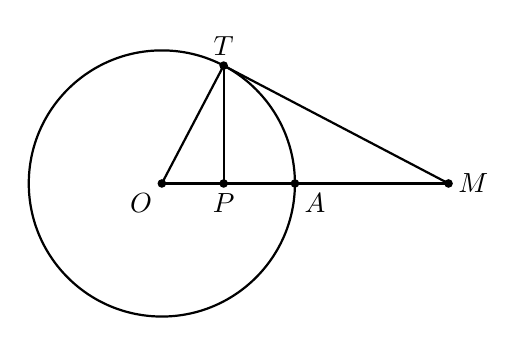
\begin{tikzpicture}[scale=1.3]
  \coordinate (O) at (0,0);
  \coordinate (M) at (2.8,0);
  \coordinate (A) at (1.3,0);
  \coordinate (P) at (0.6036,0);
  \coordinate (T) at (0.6036,1.1514);
  \draw[thick] (O) circle (1.3);
  \draw[thick] (O) -- (M);
  \draw[thick] (O) -- (T);
  \draw[thick] (T) -- (M);
  \draw[thick] (T) -- (P);
  \fill (O) circle (1.2pt) node[below left] {$O$};
  \fill (P) circle (1.2pt) node[below] {$P$};
  \fill (A) circle (1.2pt) node[below right] {$A$};
  \fill (M) circle (1.2pt) node[right] {$M$};
  \fill (T) circle (1.2pt) node[above] {$T$};
\end{tikzpicture}
\end{center}
\nopagebreak[4]
\textbf{附加题 1．（10 分）} 如果二次方程 $(m+1)x^2+(2m-1)x+(m-1)=0$ 无实数根，求证：二次方程 $(m-3)x^2-2(m+3)x-(m+5)=0$ 一定有两个不相等的实根。

\textbf{附加题 2．（10 分）} $\triangle ABC$ 的面积为 $10\sqrt3$，周长为 $20$，并且三个内角成等差数列，求各边的长。

\Needspace{4\baselineskip}
\textbf{解析}

\Needspace{5\baselineskip}
$MT$ 切 $\odot O$ 于 $T$，故 $OT\perp MT$，$\triangle OTM$ 是以 $T$ 为直角顶点的直角三角形，斜边 $OM$。因 $A$ 在 $\odot O$ 上且在线段 $OM$ 上，$OA=r$；又 $MA=h$，故

\nopagebreak[4]
\[
OM=OA+AM=r+h.
\]

\Needspace{5\baselineskip}
由勾股定理，

\nopagebreak[4]
\[
MT=\sqrt{OM^2-OT^2}=\sqrt{(r+h)^2-r^2}=\sqrt{h^2+2rh}.
\]

\Needspace{5\baselineskip}
$TP$ 是直角三角形斜边 $OM$ 上的高，故

\nopagebreak[4]
\[
TP=\frac{OT\cdot MT}{OM}=\frac{r\sqrt{h^2+2rh}}{r+h}.
\]
\nopagebreak[4]
\begin{center}% 1977 年江苏苏州市初试卷第 6 题：MT 是 ⊙O 的切线，T 为切点，
% O、P、A、M 依次在同一直线上，TP⊥MO 交于 P（按源卷第 3 页布局）
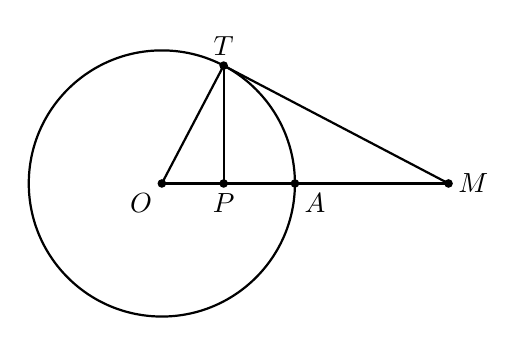
\begin{tikzpicture}[scale=1.3]
  \coordinate (O) at (0,0);
  \coordinate (M) at (2.8,0);
  \coordinate (A) at (1.3,0);
  \coordinate (P) at (0.6036,0);
  \coordinate (T) at (0.6036,1.1514);
  \draw[thick] (O) circle (1.3);
  \draw[thick] (O) -- (M);
  \draw[thick] (O) -- (T);
  \draw[thick] (T) -- (M);
  \draw[thick] (T) -- (P);
  \fill (O) circle (1.2pt) node[below left] {$O$};
  \fill (P) circle (1.2pt) node[below] {$P$};
  \fill (A) circle (1.2pt) node[below right] {$A$};
  \fill (M) circle (1.2pt) node[right] {$M$};
  \fill (T) circle (1.2pt) node[above] {$T$};
\end{tikzpicture}
\end{center}
\nopagebreak[4]
\textbf{附加题 1}

\Needspace{5\baselineskip}
方程 $(m+1)x^2+(2m-1)x+(m-1)=0$（$m\ne-1$，为二次方程）无实数根，其判别式

\nopagebreak[4]
\[
\Delta_1=(2m-1)^2-4(m+1)(m-1)=4m^2-4m+1-4(m^2-1)=5-4m<0,
\]

故 $m>\dfrac54$。

\Needspace{5\baselineskip}
方程 $(m-3)x^2-2(m+3)x-(m+5)=0$ 的判别式

\nopagebreak[4]
\[
\Delta_2=[2(m+3)]^2+4(m-3)(m+5)
=4(m^2+6m+9)+4(m^2+2m-15)
=8m^2+32m-24.
\]

\Needspace{5\baselineskip}
将 $\Delta_2$ 看作 $m$ 的二次函数，其对称轴在 $m=-2$，在 $m>\dfrac54$ 的范围内单调递增；代入 $m=\dfrac54$：

\nopagebreak[4]
\[
\Delta_2=8\left(\frac{25}{16}+5-3\right)=8\times\frac{57}{16}=\frac{57}2>0,
\]

故当 $m>\dfrac54$ 时恒有 $\Delta_2>0$，即该方程有两个不相等的实根。

\begin{gktip}
\textbf{附注}：$m=3$ 满足 $m>\dfrac54$，但此时二次项系数 $m-3=0$，方程退化为一次方程 $-12x-8=0$（仅一个实根）。原题以「二次方程」指称该式，本文按此前提证明 $m\ne3$ 时判别式恒正；$m=3$ 为该前提之外的退化情形，特此注明。
\end{gktip}

\textbf{附加题 2}

设 $\triangle ABC$ 三内角成等差数列，中间角为 $B$，则 $2B=A+C$，又 $A+B+C=180^\circ$，代入得 $3B=180^\circ$，$B=60^\circ$。

\Needspace{5\baselineskip}
由面积公式，

\nopagebreak[4]
\[
S=\frac12ac\sin B=\frac{\sqrt3}4ac=10\sqrt3
\;\Longrightarrow\;
ac=40.
\]

\Needspace{5\baselineskip}
设 $a+c=s$，由周长 $a+b+c=20$ 得 $s=20-b$。由余弦定理，

\nopagebreak[4]
\[
b^2=a^2+c^2-2ac\cos B=(a+c)^2-2ac-ac=s^2-3ac=(20-b)^2-120.
\]

\Needspace{5\baselineskip}
展开：

\nopagebreak[4]
\[
b^2=400-40b+b^2-120
\;\Longrightarrow\;
40b=280
\;\Longrightarrow\;
b=7.
\]

\Needspace{5\baselineskip}
故 $a+c=13$，$ac=40$，$a,c$ 是方程 $t^2-13t+40=0$ 的两根：

\nopagebreak[4]
\[
t=\frac{13\pm3}2=8\ \text{\text{或}}\ 5.
\]

所以三边长为 $5$、$7$、$8$（$7$ 边所对的角为 $60^\circ$）。验证：面积 $=\dfrac12\times5\times8\times\sin60^\circ=20\times\dfrac{\sqrt3}2=10\sqrt3$，周长 $5+7+8=20$，均满足题设。

\gkanswer{答案：$TP=\dfrac{r\sqrt{h^2+2rh}}{r+h}$。}

\end{answer}